\section{Triangulatie}
Wanneer de schermen herkent en geïdentificeerd zijn, worden ze aan elkaar gelinkt door middel van een triangulatie. Het project gebruikt een Delaunay triangulatie. Dit is een speciale vorm waarbij de kleinste hoek gemaximaliseert wordt en waarbij de driehoeken niet overlappen. \cite{delaunaywiki}
Er wordt gebruik gemaakt van het Bowyer-Watson algoritme. \cite{Bowyer-WatsonWiki} Het heeft een tijdscomplexiteit van $O(n^2)$, dit is zeker niet de beste complexiteit om een Delaunay triangulatie te berekenen. Aangezien in de toepassing maximaal 120 schermen gebruikt kunnen worden, voldoet $O(n^2)$. Met de eenvoudige implementatie is dit dan ook een voordehandliggende keuze.

\subsection{Bowyer-Watson}
Bowyer-Watson gaat er van uit dat punten enkel worden toegevoegd in een al bestaande Delaunay triangulatie. Als eerste worden er twee superdriehoeken gezocht. Deze driehoeken zullen alle te trianguleren punten bevatten. De implementaties waarop het algoritme is gebaseerd \cite{Bowyer-WatsonWiki} \cite{bowyer-watsonImplementation} stelden beiden een `superdriehoek' voor, zie figuur \ref{bowyer-watson-a} Echter is het eenvoudiger om een omkaderende vierhoek te vormen en deze op te delen in twee driehoeken. Vervolgens worden alle punten één voor één toegevoegd.

Voor elk punt worden alle driehoeken gezocht waarvan het punt in de omschreven cirkel zit. Wanneer twee driehoeken eenzelfde zijde delen, wordt deze verwijderd. Alle punten van de omschreven veelhoek van de twee driehoeken worden nu verbonden met het toegevoegde punt, zie figuur \ref{bowyer-watson-b}. Met deze werkwijze zal er op elk moment een Delaunay triangulatie zijn en moeten de driehoeken achteraf niet meer overlopen worden. Met het gevolg dat het data management voor deze methode minder complex is.

Eens alle punten toegevoegd zijn, worden de driehoeken die één of meer hoeken van de omkaderende vierhoek bevatten verwijderd, zie figuur \ref{bowyer-watson-c}. Aangezien deze driehoeken aan de buitenkant liggen is dit toegestaan. Er zal een Delaunay triangulatie overblijven van alle onderzochte punten.

\begin{figure}[H]
	\center
	\begin{subfigure}{0.4\textwidth}
		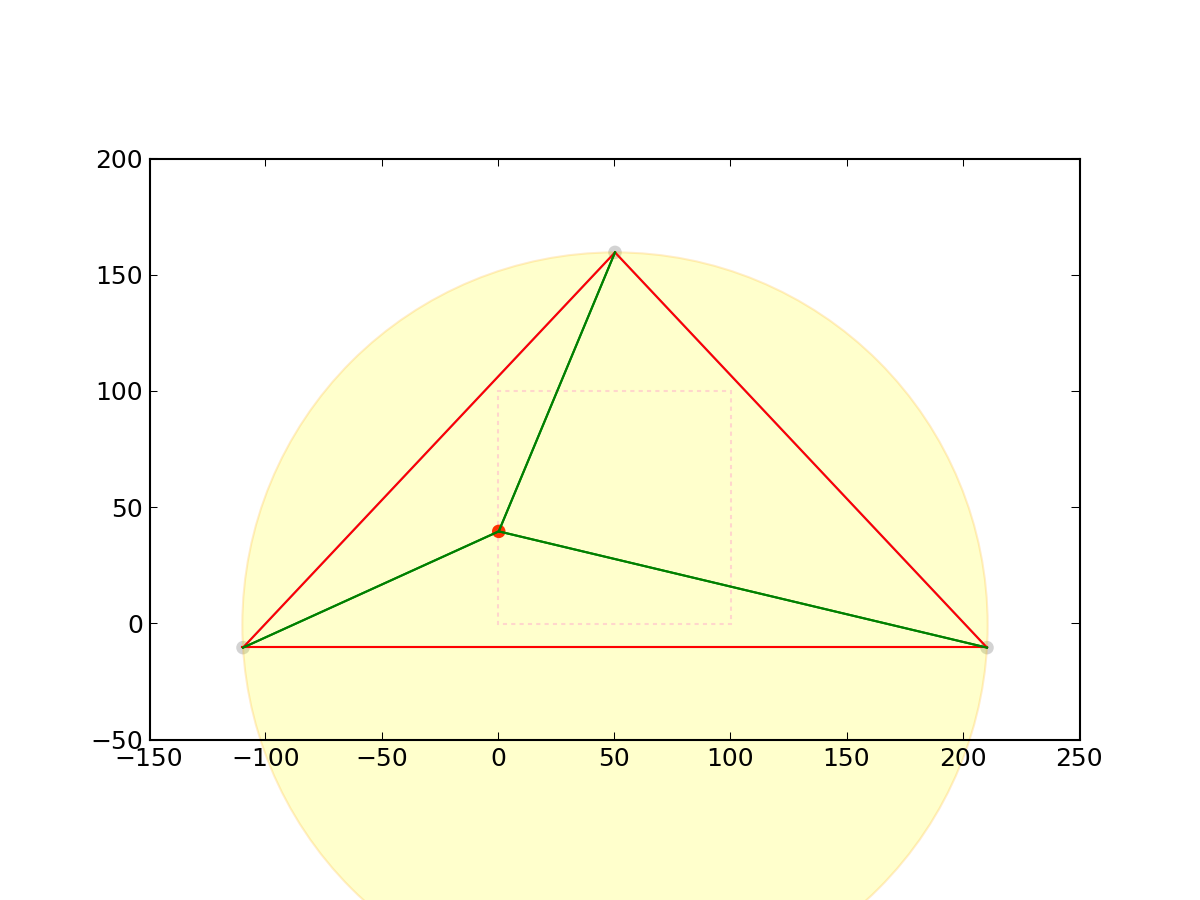
\includegraphics[width=\textwidth]{img/bowyer-watson_superdriehoek}
		\caption{De rode superdriehoek waarin alle punten zullen worden toegevoegd.}
		\label{bowyer-watson-a}
	\end{subfigure}
	\begin{subfigure}{0.4\textwidth}
		\includegraphics[width=\textwidth]{img/bowyer-watson_nieuwpunt}
		\caption{Een nieuw punt wordt toegevoegd. In geel de omschreven cirkels. De gestippelde zijde wordt verwijderd, de groene toegevoegd.}
		\label{bowyer-watson-b}
	\end{subfigure}
		\begin{subfigure}{0.4\textwidth}
		\includegraphics[width=\textwidth]{img/bowyer-watson_verwijderen}
		\caption{In rood alle driehoeken verbonden met de superdriehoek, deze worden uiteindelijk verwijderd.}
		\label{bowyer-watson-c}
	\end{subfigure}
	\caption{Het Bowyer-Watson algoritme \cite{Bowyer-WatsonWiki}}
	\label{bowyer-watson}
\end{figure}

\subsection{Valkuilen}
In theorie kan er van elke opstelling waarbij de punten niet allemaal colineair zijn een triangulatie worden gevonden, zie figuur \ref{colineair}. Echter door afronding bij de berekeningen zal er bij bijna colineaire punten geen juiste  configuratie gevonden worden, zie figuur \ref{almost_colineair}. 

\begin{figure}[H]
	\center
	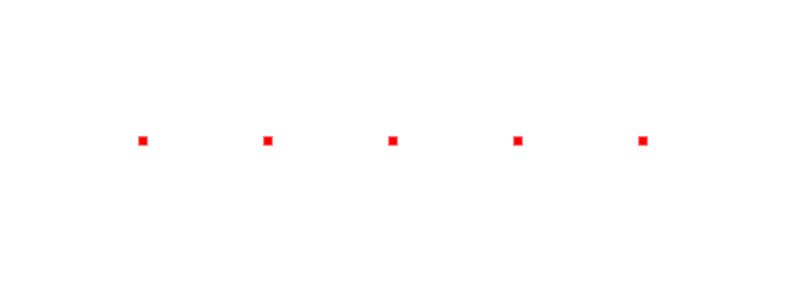
\includegraphics[width=0.4\textwidth]{img/colineair}
	\caption{Van colineaire punten kan geen triangulatie gevonden worden.}
	\label{colineair}
\end{figure}
\begin{figure}[H]
	\center
	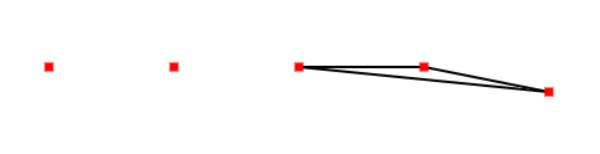
\includegraphics[width=0.4\textwidth]{img/almost_colinair}
	\caption{Van bijna colineaire punten kan geen triangulatie gevonden worden door afrondingsfouten bij berekeningen.}
	\label{almost_colineair}
\end{figure}

